\chapter{Sygnał dźwiękowy i~podstawy teorii muzyki} \label{chapter:music_theory}
\chaptermark{Sygnał dźwiękowy i~teoria muzyki}

Niniejszy rozdział zawiera wprowadzenie teoretyczne, niezbędne do zrozumienia koncepcji akordu i~wykorzystanych algorytmów wstępnego przetwarzania utworów muzycznych. Po pierwsze przedstawione zostały absolutne podstawy z~obszaru cyfrowego przetwarzania sygnałów, czyli DSP (ang. \emph{Digital Signal Processing}), ponieważ przetwarzanie dźwięku za pomocą komputera stanowi właśnie formę cyfrowego przetwarzania sygnału. Dalej wprowadzony został szereg pojęć z~teorii muzyki, zmierzający do wyjaśnienia czym właściwie jest akord muzyczny. Na końcu dodany został krótki opis nieskomplikowanego, historycznego już, najbardziej podstawowego algorytmu automatycznego rozpoznawania akordów muzycznych.



\section{Podstawy cyfrowego przetwarzania sygnałów}

Sygnał dźwiękowy może być opisany jako zmiany poziomu ciśnienia akustycznego w~funkcji czasu\footnote{\cite{lerch_introduction_2012}, s. 7}. W~praktyce oznacza to okresowe drganie cząsteczek powietrza lub innego ośrodka, które rozchodzi się w~postaci fali (dźwiękowej) i~może zostać zarejestrowane przez narząd słuchu. Aby było to możliwe, parametry sygnału dźwiękowego muszą mieścić się w określonym zakresie. Różne stworzenia posiadają różne granice słyszalności i~tak np. pies jest w~stanie usłyszeć dźwięki, których człowiek nie potrafi w żaden sposób zauważyć. 

Będący tematem tego rozdziału sygnał dźwiękowy (określany również po prostu jako \emph{dźwięk}) posiada wiele parametrów i~może podlegać najróżniejszym analizom i~przekształceniom.  Oczywiście sygnał dźwiękowy może pochodzić z~różnych źródeł i~analizowanie tego sygnału może mieć wszelakie cele, od rozpoznawania zbliżającej się straży pożarnej, poprzez rozpoznawanie mowy, aż do analizy utworu muzycznego i~konkretnych jego cech. Z~punktu widzenia niniejszej pracy to właśnie ten ostatni przypadek jest istotny i~wszelkie operacje przetwarzania sygnału będą dokonywane na fragmentach utworów muzycznych.

% sygnał cyfrowy - próbkowanie i~kwantyzacja
Ponieważ tworzony w~ramach tej pracy system działa w środowisku cyfrowym, niemożliwa jest tam idealnie zgodna z~rzeczywistością reprezentacja sygnału dźwiękowego. W~praktyce wykorzystywana do przetwarzania jest jego cyfrowa reprezentacja, która ma formę dyskretną zarówno co do czasu, jak i~co do amplitudy. Zatem przed właściwym przystąpieniem do przetwarzania sygnału dźwiękowego, podczas procesu rejestracji za pomocą dedykowanego urządzenia --- mikrofonu, który zamienia zmiany ciśnienia akustycznego na zmiany napięcia, sygnał ulega dwóm przekształceniom, przedstawionym na rys.  \ref{fig:probkowanie_i_kwantyzacja}. Pierwsze to \emph{próbkowanie}\footnote{\cite{lerch_introduction_2012}, s. 9} z~pewną częstotliwością $f_p$, polegające na tym, że czas ulega dyskretyzacji i~z ciągłego sygnału dźwiękowego zapisane są jedynie niektóre wartości, równomiernie oddalone od siebie o $T_s=1/f_p$ sekundy. Po drugie \emph{kwantyzacja}\footnote{\cite{lerch_introduction_2012}, s. 11}, czyli zaokrąglenie wartości amplitudy do najbliższej z~wcześniej zdefiniowanego zbioru $N$ możliwych wartości. Liczba dozwolonych wartości amplitudy determinuje liczbę $w$ bitów pamięci komputera potrzebnych na zapisanie pojedynczej próbki sygnału, zgodnie ze wzorem $w=\log_{2}N$.

\begin{figure}[htb]
    \centering
    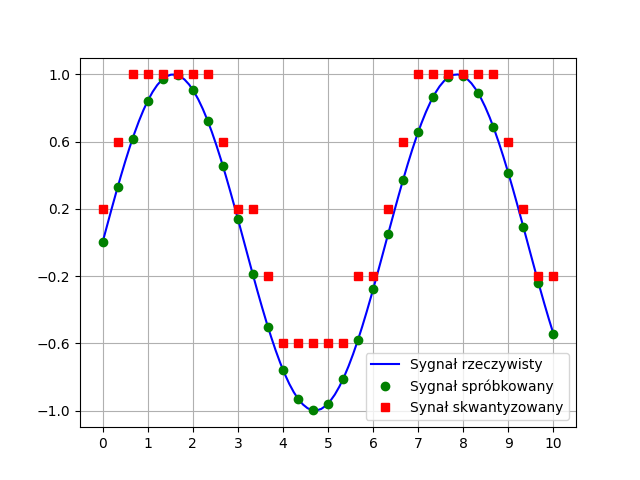
\includegraphics[width=0.9\textwidth]{images/probkowanie_i_kwantyzacja}
    \caption{Operacje próbkowania i~kwantyzacji.}
    \label{fig:probkowanie_i_kwantyzacja}
\end{figure}

% sygnał okresowy i~losowy
Sygnał dźwiękowy może być \emph{sygnałem okresowym} lub \emph{sygnałem losowym}\footnote{\cite{lerch_introduction_2012}, s. 7-8}. Pierwszy z~nich powtarza się co określony odcinek czasu $T_0$, a~drugi nie jest przewidywalny i~jego wartości są zupełnie losowe. Przykładem pierwszego z~nich jest dźwięk pianina, przedstawiony na rys \ref{fig:sygnal_okresowy}, gdzie da się dostrzec widoczną powtarzalność pewnego odcinka sygnału.  Sygnał losowy w~postaci tzw. białego szumu został przedstawiony na rys. \ref{fig:sygnal_losowy}.

\begin{figure}[htb]
    \centering
    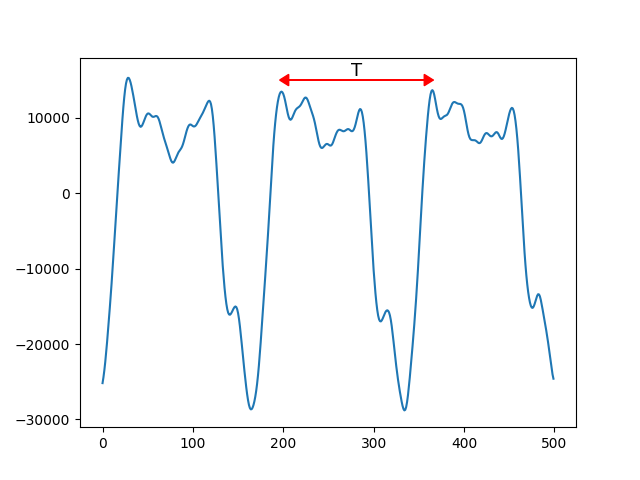
\includegraphics[width=0.9\textwidth]{images/sygnal_okresowy}
    \caption{Przykładowy sygnał okresowy --- pojedynczy dźwięk pianina.}
    \label{fig:sygnal_okresowy}
\end{figure}

\begin{figure}[htb]
    \centering
    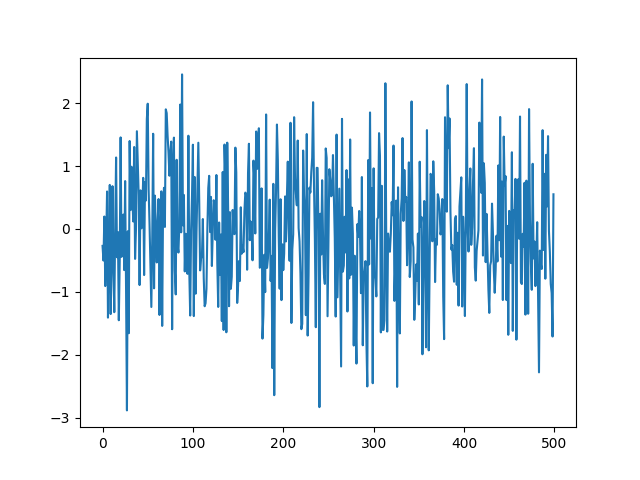
\includegraphics[width=0.9\textwidth]{images/sygnal_losowy}
    \caption{Przykładowy sygnał losowy --- biały szum.}
    \label{fig:sygnal_losowy}
\end{figure}

% częstotliwości składowe
Sygnał losowy jest mniej istotny z~punktu widzenia tej pracy. Ma on swoje miejsce w~muzyce i~niektóre instrumenty (zwłaszcza perkusyjne) mogą być jego źródłem. Jednakże, aby dało się we fragmencie sygnału dźwiękowego wyróżnić akord, musi to być sygnał okresowy. Na rys. \ref{fig:probkowanie_i_kwantyzacja} oryginalny sygnał jest \emph{tonem prostym}. Oznacza to, że zawiera on w~sobie tylko jedną \emph{częstotliwość składową}, którą da się tam wyraźnie zauważyć. W~przyrodzie właściwie nie występują tony proste. Różne odgłosy przyrody ożywionej i~nieożywionej, dźwięki instrumentów czy ludzki głos zawsze posiadają więcej częstotliwości składowych, tworzących dany sygnał. Widać to na rys. \ref{fig:sygnal_okresowy}, gdzie przedstawiono fragment sygnału dźwiękowego pochodzącego z~pianina. Da się tutaj gołym okiem zauważyć najniższą częstotliwość składową, tzw. \emph{częstotliwość podstawową} (odpowiadający jej okres jest zaznaczony czerwoną strzałką). Nie jest to jednak jedyna częstotliwość obecna w~tym sygnale i~fakt, że wykres ten jest tak ,,pofalowany'' to właśnie skutek obecności innych, wyższych składowych. Składowe te decydują o~barwie i~charakterze dźwięku, sprawiają, że jesteśmy w~stanie rozróżnić między sobą różne instrumenty czy też różnych mówców, chociażby wydawali z~siebie dźwięk o~tej samej częstotliwości podstawowej. 

% DFT
Podstawowym narzędziem pozwalającym wyróżnić częstotliwości składowe sygnału, czyli uzyskać jego \emph{widmo}, jest \emph{Transformacja Fouriera}\footnote{\cite{lyons_wprowadzenie_2000}, s. 61}. Oryginalnie jest ona zdefiniowana dla sygnału ciągłego, ale istnieje również jej dyskretna wersja, w~skrócie DFT (ang. \emph{Discrete Fourier Transform}). Przekształca ona sygnał $x$ o~długości $N$ w~sygnał $X$ o~tej samej długości, zgodnie ze wzorem:
\begin{equation} \label{eq:dft}
    X(k) = \sum_{n=0}^{N-1} x(n) e^{-ink \frac{2 \pi}{N}}
\end{equation}
gdzie $k$ to numer próbki sygnału wyjściowego $X$ (odpowiadającej pojedynczej częstotliwości), $n$ to numer próbki sygnału wejściowego $x$, a $i$ to jednostka urojona.

% STFT
Czasami stosuje się również pojęcie STFT (ang. \emph{Short Time Fourier Transform})\footnote{\cite{lerch_introduction_2012}, s. 20}, które właściwie oznacza to samo co DFT, tylko odnosi się do dłuższego fragmentu sygnału, który dzieli się na bloki i~dopiero dla każdego z~nich wykonuje się DFT. Wynik STFT jest więc macierzą, gdzie każda kolumna zawiera wynik DFT dla pojedynczego bloku (ramki) sygnału. Jeżeli sygnał jest próbkowany z~częstotliwością $f_s$, to wtedy wartość $k$ sygnału wynikowego $X$ informuje o~fazie i~natężeniu składowej o~częstotliwości $f(k) = \frac{f_s}{N}k$.  Oczywiście, jak widać we wzorze \ref{eq:dft}, wynik transformacji Fouriera ma postać zespoloną. Aby uzyskać natężenie danej składowej należy wziąć wartość bezwzględną liczby zespolonej, jej argument informuje natomiast o~przesunięciu fazowym danej składowej. Na rys.  \ref{fig:transformata_fouriera} przedstawiono wynik przeprowadzenia opisanych powyżej operacji na dwóch przykładowych sygnałach --- tonie prostym o~jednej częstotliwości składowej i~bardziej złożonym sygnale, będącym złożeniem trzech częstotliwości. Warto jeszcze zaznaczyć, że jeżeli sygnał wejściowy ma wartości rzeczywiste, to wynik DFT jest symetryczny\footnote{\cite{lyons_wprowadzenie_2000}, s. 72} i~dlatego uwzględnia się tylko jego pierwszą połowę.

\begin{figure}[htb]
    \centering
    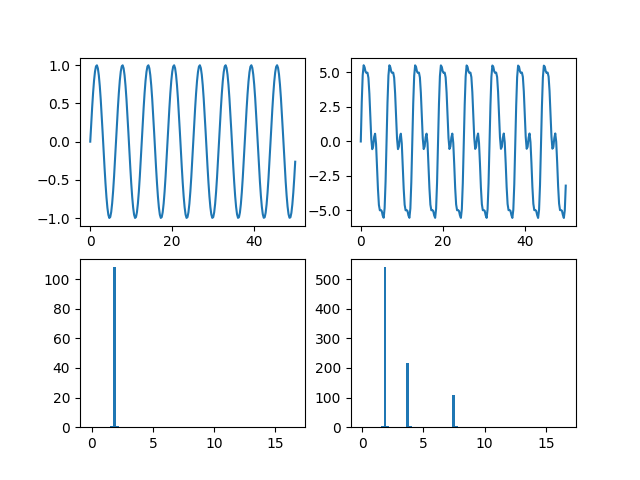
\includegraphics[width=0.9\textwidth]{images/transformata_fouriera}
    \caption{Wyniki Transformacji Fouriera (dolny rząd) dla dwóch przykładowych sygnałów (górny rząd).}
    \label{fig:transformata_fouriera}
\end{figure}

% FFT
W~praktyce nie wylicza się DFT bezpośrednio ze wzoru, ponieważ wiąże się to z~kwadratową złożonością obliczeniową, co zupełnie uniemożliwia przetwarzanie w~czasie rzeczywistym. Korzysta się z~szybkiej wersji algorytmu o~nazwie FFT (ang. \emph{Fast Fourier Transform})\footnote{\cite{lyons_wprowadzenie_2000}, s. 132}, którego omówienie wykracza poza zakres tej pracy.

% funkcje okna
Jeżeli składowe sygnału poddawanego transformacji Fouriera nie pokrywają się idealnie z~częstotliwościami odpowiadającymi poszczególnym punktom transformaty, dochodzi do \emph{przecieku}\footnote{\cite{lyons_wprowadzenie_2000}, s. 80}. Polega on na tym, że energia takiej składowej uwidacznia się we wszystkich wartościach wyniku DFT. Aby minimalizować to zjawisko, stosuje się \emph{funkcje okna}. Jest to funkcja, którą stosuje się dla fragmentu sygnału o~długości $N$ próbek, przed przeprowadzeniem na nim DFT. Przykładową funkcją okna jest \emph{okno Hanninga}, które wyraża się wzorem:
\begin{equation}
    f(n) = 0.5 - 0.5 \cos (2 \pi n / N)
\end{equation}
gdzie $n$ jest numerem próbki sygnału a $N$ liczbą próbek.

% spektrogramy
Do przeprowadzenia analizy widma (czyli częstotliwości składowych) fragmentu pewnego sygnału, DFT nadaje się idealnie. Jednakże utwory muzyczne w~muzyce popularnej trwają zazwyczaj kilka minut i~podczas ich analizy bardzo ważne jest, aby uwzględnić zmiany dźwięków w~czasie. Sam wynik DFT nie niesie żadnej informacji o~zmianach częstotliwości składowych, jedynie o~ich obecności, fazie i~natężeniu.  W~praktyce reprezentuje się więc sygnał dźwiękowy w~postaci \emph{spektrogramu}\footnote{\cite{lerch_introduction_2012}, s. 21}, który jest dwuwymiarową reprezentacją dźwięku i~zawiera informację o~natężeniu częstotliwości składowych sygnału w~kolejnych chwilach czasu. Aby utworzyć taki spektrogram, którego przykład został zaprezentowany na rys.  \ref{fig:spektrogram}, należy podzielić sygnał na niewielkie, trwające np. ułamek sekundy części. Na każdej z~nich przeprowadza się DFT, wylicza moduł wartości zespolonych i~ostatecznie otrzymuje się natężenie częstotliwości składowych dla każdego z~wydzielonych kawałków. Właściwie jest to więc wspomniana wcześniej operacja STFT, która jest jednym ze sposobów tworzenia spektrogramu. Czym wyższa wartość w~spektrogramie, prezentowana zazwyczaj poprzez jaśniejszy kolor, tym głośniejsza jest dana częstotliwość składowa w~danej chwili czasu.

\begin{figure}[htb]
    \centering
    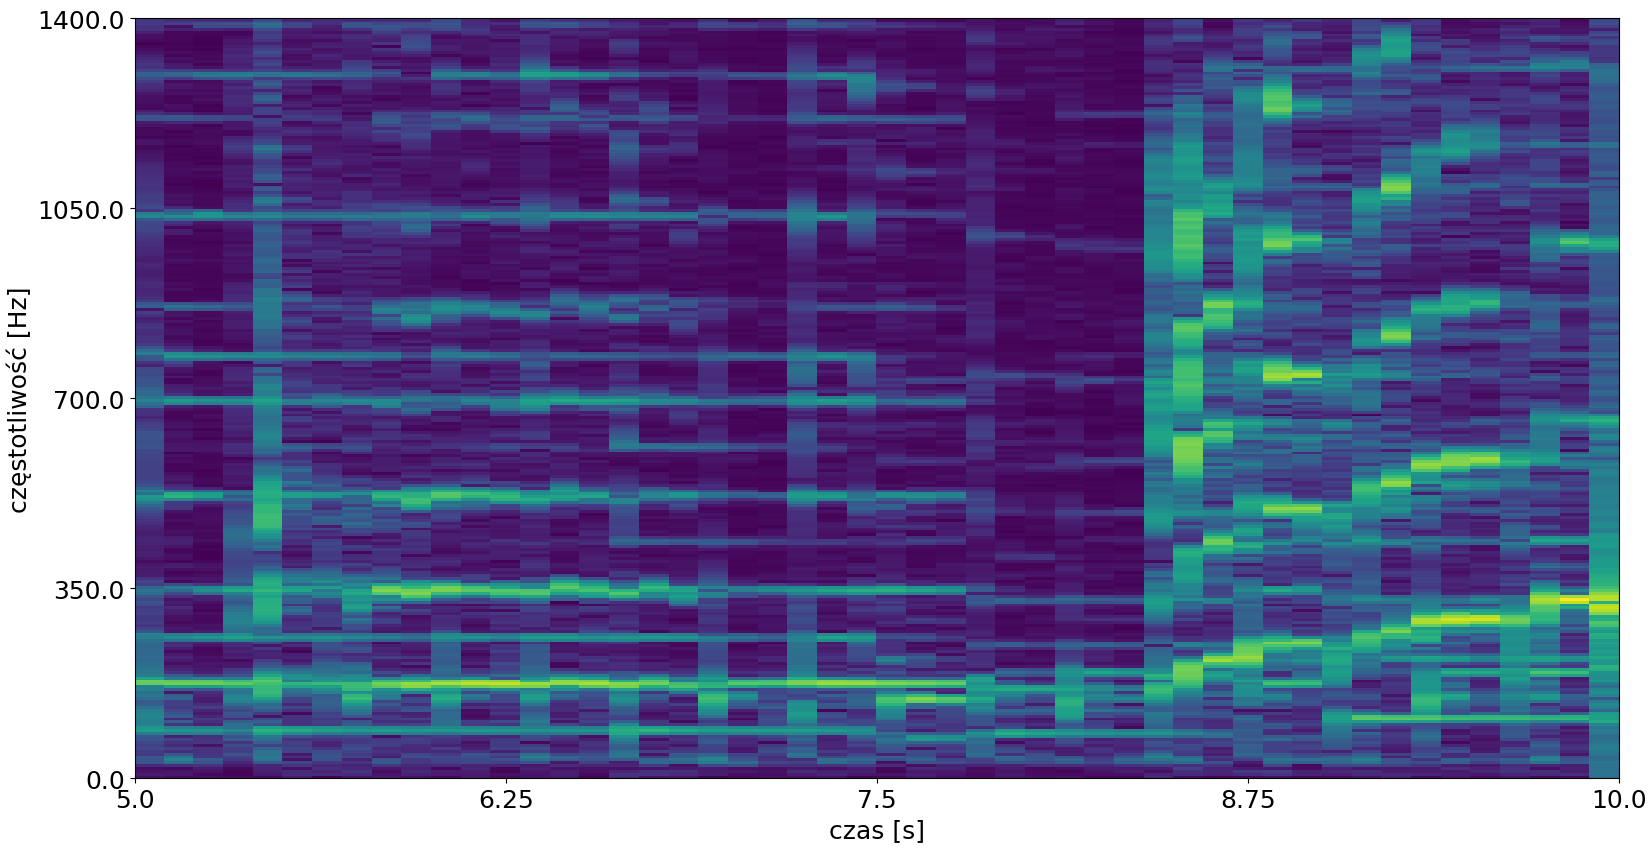
\includegraphics[width=0.9\textwidth]{images/spektrogram}
    \caption{Przykładowy spektrogram (fragment piosenki ,,Yesterday'' zespołu The Beatles).}
    \label{fig:spektrogram}
\end{figure}



\section{Podstawy teorii muzyki}

% głośność i~wysokość
Zanim omówione zostaną niezbędne pojęcia z~teorii muzyki, należy wspomnieć o~tym, jak ludzkie ucho odbiera i~interpretuje sygnał dźwiękowy. Posiada on dwie podstawowe cechy: \emph{głośność}\footnote{\cite{lerch_introduction_2012}, s. 71}, która jest związana z~amplitudą sygnału, oraz \emph{wysokość}\footnote{\cite{lerch_introduction_2012}, s. 79}, która zależy od częstotliwości. Czym większa amplituda tym dźwięk jest głośniejszy i~czym wyższa częstotliwość, tym dźwięk jest wyższy. Warto zwrócić uwagę, że zależność pomiędzy wrażeniem głośności i~wysokości, a~faktycznymi, liczbowymi wartościami amplitudy i~częstotliwości jest logarytmiczna. Oznacza to, że aby subiektywna głośność dźwięku zwiększała się w~sposób jednostajny, to jego amplituda musi rosnąć wykładniczo, to samo odnosi się do wysokości dźwięku. 

% dźwięki o~określonej wysokości
Jeżeli częstotliwości składowe pojedynczego dźwięku, są kolejnymi wielokrotnościami częstotliwości podstawowej, to wtedy da się wyraźnie zauważyć, że dźwięk taki ma określoną wysokość i~odpowiada ona właśnie częstotliwości podstawowej\footnote{\cite{lerch_introduction_2012}, s. 79}. Oznacza to, że pojedynczy dźwięk pianina, trąbki czy gitary składa się z~bardzo wielu częstotliwości ułożonych zgodnie z~opisaną wyżej regułą. Oczywiście istnieją również dźwięki, gdzie układ ten nie jest zachowany. Wtedy trudno jest jednak lub czasem zupełnie niemożliwe, aby określić wysokość dla takiego dźwięku. Rys. \ref{fig:spektrogram_c} przedstawia spektrogram pojedynczego dźwięku zagranego na pianinie. Dźwięk ten ma pojedynczą, określoną wysokość, jednakże posiada wiele częstotliwości składowych. Wszystkie one są wielokrotnościami częstotliwości podstawowej, co wyraźnie da się zauważyć na podstawie regularnego układu jasnych linii na rysunku.

\begin{figure}[htb]
    \centering
    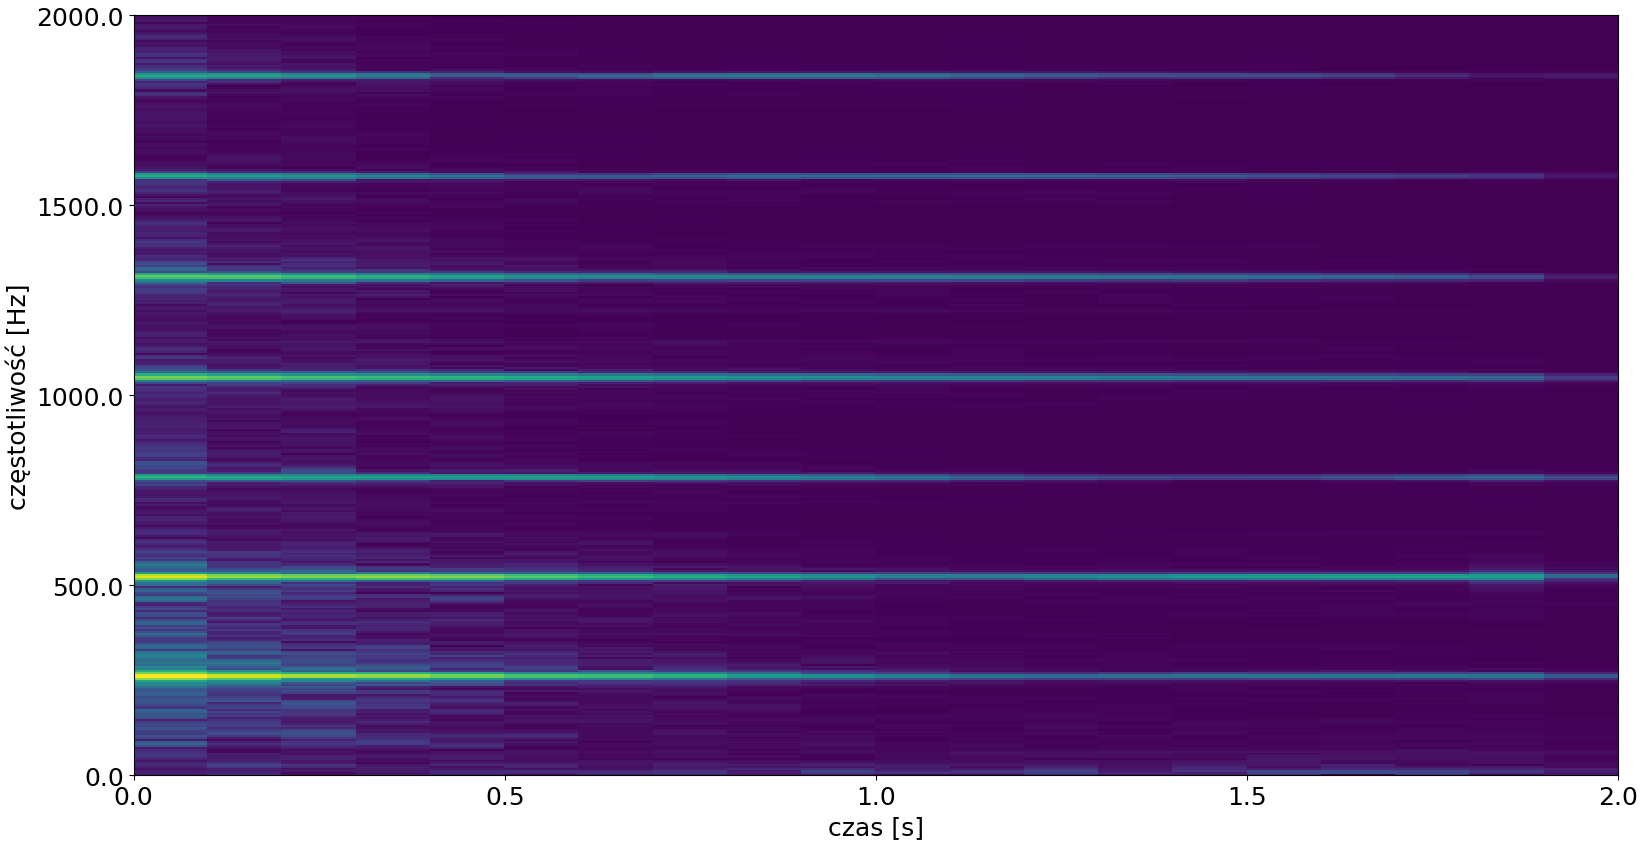
\includegraphics[width=0.9\textwidth]{images/spektrogram_c}
    \caption{Spektrogram pojedynczego dźwięku C~zagranego na pianinie.}
    \label{fig:spektrogram_c}
\end{figure}

% oktawy, 12 dźwięków i~strój równomiernie temperowany
Istnieje jeszcze jedno istotne zjawisko, związane z~ludzką percepcją sygnału dźwiękowego. Mianowicie nasz mózg rozpoznaje jako bardzo podobne do siebie, te dźwięki, których stosunek częstotliwości podstawowych jest potęgą dwójki\footnote{\cite{lerch_introduction_2012}, s. 81}. Ma to bezpośredni wpływ na nazewnictwo dźwięków. Tą samą nazwą literową oznaczone zostały właśnie te dźwięki, których stosunek częstotliwości podstawowych jest potęgą dwójki. Odległość między dwoma najbliższymi dźwiękami o~tej samej nazwie, czyli takimi, których stosunek częstotliwości jest równy $2:1$, nazywa się \emph{oktawą}. Przyjęto, że pomiędzy taką parą dźwięków, czyli w~ramach pojedynczej oktawy, mieści się jeszcze jedenaście innych dźwięków. W~ten sposób dochodzimy do stwierdzenia, że w~muzyce wyróżnia się dwanaście różnych nazw dźwięków, które są oddalone od siebie o~odległość \emph{półtonu}. Każda z~tych dwunastu nazw odpowiada zatem wielu częstotliwościom podstawowym. Odległość półtonu jest natomiast najmniejszą odległością pomiędzy dźwiękami, jaką stosuje się w~muzyce popularnej ,,cywilizacji zachodniej''. Zauważmy, że --- z~uwagi na wspomnianą wcześniej logarytmiczną zależność subiektywnej wysokości dźwięku od jego częstotliwości --- różnica częstotliwości odpowiadająca odległości jednego półtonu rośnie wraz ze zwiększeniem się wartości częstotliwości, w~obrębie których się poruszamy. System, w~którym częstotliwości podstawowe kolejnych dźwięków w~oktawie rozłożone są ,,równomiernie'', to znaczy stosunek częstotliwości podstawowych $f_1$ i $f_2$ dowolnych dwóch dźwięków oddalonych od siebie o $N$ półtonów jest zawsze taki sam i~wynosi:
\begin{equation} \label{eq:stroj_rownomiernie_temperowany}
    \frac{f_1}{f_2} = 2^{N/12}
\end{equation}
nazywany jest \emph{strojem równomiernie temperowanym}\footnote{\cite{lerch_introduction_2012}, s. 90}. Jest to podstawowy strój stosowany dziś w~muzyce zachodniej. Istnieją również inne systemy, ale ich omówienie wykracza poza zakres niniejszej pracy.

% nazwy dźwięków, modyfikatory
Aby móc określić częstotliwości podstawowe odpowiadające danym nazwom dźwięków, trzeba zdefiniować pewną częstotliwość wzorcową (\emph{częstotliwość strojenia}\footnote{\cite{lerch_introduction_2012}, s. 88}). Często przyjmuje się za nią $440$ Hz, która to częstotliwość odpowiada dźwiękowi oznaczanemu literą ,,A''. Wykorzystując wspomnianą częstotliwość i~zakładając, że poruszamy się w~ramach stroju równomiernie temperowanego, na podstawie wzoru \ref{eq:stroj_rownomiernie_temperowany} można wyliczyć jakie częstotliwości podstawowe przyjmują kolejne dźwięki. Wszystkie dwanaście nazw dźwięków muzycznych wraz z~ich oznaczeniami i~przykładowymi częstotliwościami podstawowymi (w obrębie jednej, wybranej oktawy), wyliczonymi przy wspomnianych wyżej założeniach, przedstawiono w~Tab. \ref{tab:nazwy_dzwiekow}. Zaproponowane oznaczenia bazują na \cite{lerch_introduction_2012} i~ich budowa sprowadza się do wykorzystania dwóch symboli: krzyżyka \musSharp{} oraz bemola \musFlat{}, które stosuje się również w~zapisie nutowym (który nie będzie tutaj omawiany). Pierwszy z~nich oznacza podwyższenie dźwięku o~pół tonu a~drugi obniżenie o~pół tonu. Można powiedzieć więc, że w~oznaczeniach dźwięków wykorzystuje się $7$ liter oraz $2$ symbole-modyfikatory. Zauważmy, że niektóre dźwięki można przedstawić na dwa sposoby, a~przyjmując możliwość wielokrotnego wykorzystania modyfikatorów (podwójny krzyżyk, podwójny bemol), liczba alternatywnych nazw wzrasta jeszcze bardziej. Kolejne oktawy mają swoje nazwy (mała, wielka, razkreślna itd.), które wykorzystuje się, kiedy trzeba odróżnić dwa dźwięki o~tej samej nazwie w~dwóch różnych oktawach (np. $a$ razkreślne --- $a^1$).

\begin{table}[htb]
    \centering
    \caption{Nazwy dźwięków w~muzyce.}
    \label{tab:nazwy_dzwiekow}
    \begin{tabular}{|c|c|c|} \hline
        Nazwa & Oznaczenie & Częstotliwość (jedna z~wielu) [Hz] \\ \hline
        c       & C     & $261.6$  \\
        cis/des & C\sh{}/D\fl{} & $277.2$  \\
        d       & D     & $293.7$  \\
        dis/es  & D\sh{}/E\fl{} & $311.1$  \\
        e       & E     & $329.6$  \\
        f       & F     & $349.2$  \\
        fis/ges & F\sh{}/G\fl{} & $370.0$  \\
        g       & G     & $392.0$  \\
        gis/as  & G\sh{}/A\fl{} & $415.3$  \\
        a       & A     & $440.0$  \\
        ais/b   & A\sh{}/B  & $466.2$  \\
        h       & H     & $493.9$  \\
        c       & C     & $523.2$  \\ \hline
    \end{tabular}
\end{table}

% interwały
Odległość pomiędzy dwoma dźwiękami nazywa się \emph{interwałem muzycznym}\footnote{\cite{lerch_introduction_2012}, s.  83}. Interwały składają się z całkowitych wielokrotności półtonu --- każdy kolejny interwał jest o~pół tonu większy od poprzedniego. Nazwy dwunastu pierwszych interwałów wraz z~ich oznaczeniami stosowanymi w~muzyce przedstawiono w~Tab. \ref{tab:interwaly}. Ostatni z~nich to wspomniana już wcześniej oktawa --- dźwięki oddalone od siebie o~oktawę mają tę samą nazwę. 

\begin{table}[htb]
    \centering
    \caption{Interwały muzyczne.}
    \label{tab:interwaly}
    \begin{tabular}{|c|c|c|} \hline
        Nazwa & Oznaczenie & Liczba półtonów \\ \hline
        Pryma           & 0     & 0  \\
        Sekunda mała    & 2>    & 1  \\
        Sekunda wielka  & 2     & 2  \\
        Tercja mała     & 3>    & 3  \\
        Tercja wielka   & 3     & 4  \\
        Kwarta czysta   & 4     & 5  \\
        Tryton          & 4<    & 6  \\
        Kwinta czysta   & 5     & 7  \\
        Seksta mała     & 6>    & 8  \\
        Seksta wielka   & 6     & 9  \\
        Septyma mała    & 7     & 10 \\
        Septyma wielka  & 7<    & 11 \\
        Oktawa czysta   & 8     & 12 \\ \hline
    \end{tabular}
\end{table}

% akord
Jednoczesne brzmienie więcej niż dwóch dźwięków nazywa się \emph{akordem muzycznym}\footnote{\cite{lerch_introduction_2012}, s. 86}. Składa się więc on z (przynajmniej dwóch) interwałów, które znajdują się między parami dźwięków. Zależnie od interwałów, stanowiących ich podstawowy budulec, akordy mają zupełnie różne brzmienie i~charakter. Akordy rozróżnia się więc po ich bazowym dźwięku i~po ich typie. Wyróżnić można wiele rodzajów akordów, ale na potrzeby niniejszej pracy najważniejsze są dwa z~nich.  Pierwszy to tzw. \emph{akord majorowy}, który zawiera kolejno tercję wielką i~tercję małą, a~drugi to \emph{akord minorowy}, który zawiera te same interwały, ale w~odwrotnej kolejności. Pierwszy ma charakter radosny, a~drugi smutny i~melancholijny. Zarówno akordy pierwszego, jak i~drugiego typu mogą być zbudowane na każdym z~dwunastu dźwięków. 

% dalej o~akordach
Aby zbudować akord trzeba wybrać dźwięk bazowy, czyli tzw. podstawę akordu. Dla przykładu weźmy dźwięk A. Następnie trzeba obliczyć, jakie dźwięki są oddalone o~odpowiednie interwały. Jeżeli budujemy akord majorowy, to kolejnymi dźwiękami tego akordu są C\sh{} oraz E. Jeżeli budujemy akord minorowy, to będą to C~i E. Jak widać, różnią się tylko jednym dźwiękiem. Pierwszy z~opisanych akordów nazywa się \emph{A-dur} a~drugi \emph{a-moll}. W~praktyce te trzy lub więcej dźwięków nie muszą być umieszczone w~ramach pojedynczej oktawy. Dany składnik akordu może wystąpić w~dowolnej oktawie lub nawet powtórzyć się w~dwóch lub więcej oktawach jednocześnie. Nie zawsze więc podstawa akordu jest jego najniższym dźwiękiem. To, który składnik jest najniższym dźwiękiem akordu (tzw. bas), definiuje jaki jest \emph{przewrót} danego akordu. W~przypadku prostych, trójskładnikowych akordów majorowych i~minorowych możliwe są dwa przewroty. Budowę kilku przykładowych akordów przedstawiono w~Tab. \ref{tab:przykladowe_akordy}. Jak łatwo zauważyć, nazwy akordów majorowych tworzy się poprzez dodanie sufiksu ,,dur'' do podstawy akordu, a~nazwy akordów minorowych poprzez dodanie sufiksu ,,moll''.

\begin{table}[htb]
    \centering
    \caption{Przykładowe akordy muzyczne.}
    \label{tab:przykladowe_akordy}
    \begin{tabular}{|c|c|c|} \hline
        Nazwa akordu & Nazwy dźwięków składowych \\ \hline
        A-dur   & A  C\sh{} E  \\
        g-moll  & G  B  D  \\
        Fis-dur  & F\sh{} A\sh{} C\sh{} \\
        b-moll  & B  Db F  \\ \hline
    \end{tabular}
\end{table}

Na końcu warto jeszcze podkreślić, że widmo częstotliwościowe pojedynczego akordu, nawet jeśli składa się on tylko z $3$ dźwięków, będzie kilka razy bardziej złożone niż widmo pojedynczego dźwięku. Wynika to z~faktu, że każdy dźwięk budujący akord ma poza częstotliwością podstawową wiele wyższych częstotliwości składowych. Przykładowy spektrogram zagranego na pianinie akordu C-dur zaprezentowano na rys. \ref{fig:spektrogram_cdur}. Jak widać, nie jest łatwo stwierdzić na pierwszy rzut oka, która składowa pochodzi z~którego dźwięku akordu (C, E, lub G). Zauważmy też, że dwa różne dźwięki mogą mieć te same częstotliwości niektórych składowych.

\begin{figure}[htb]
    \centering
    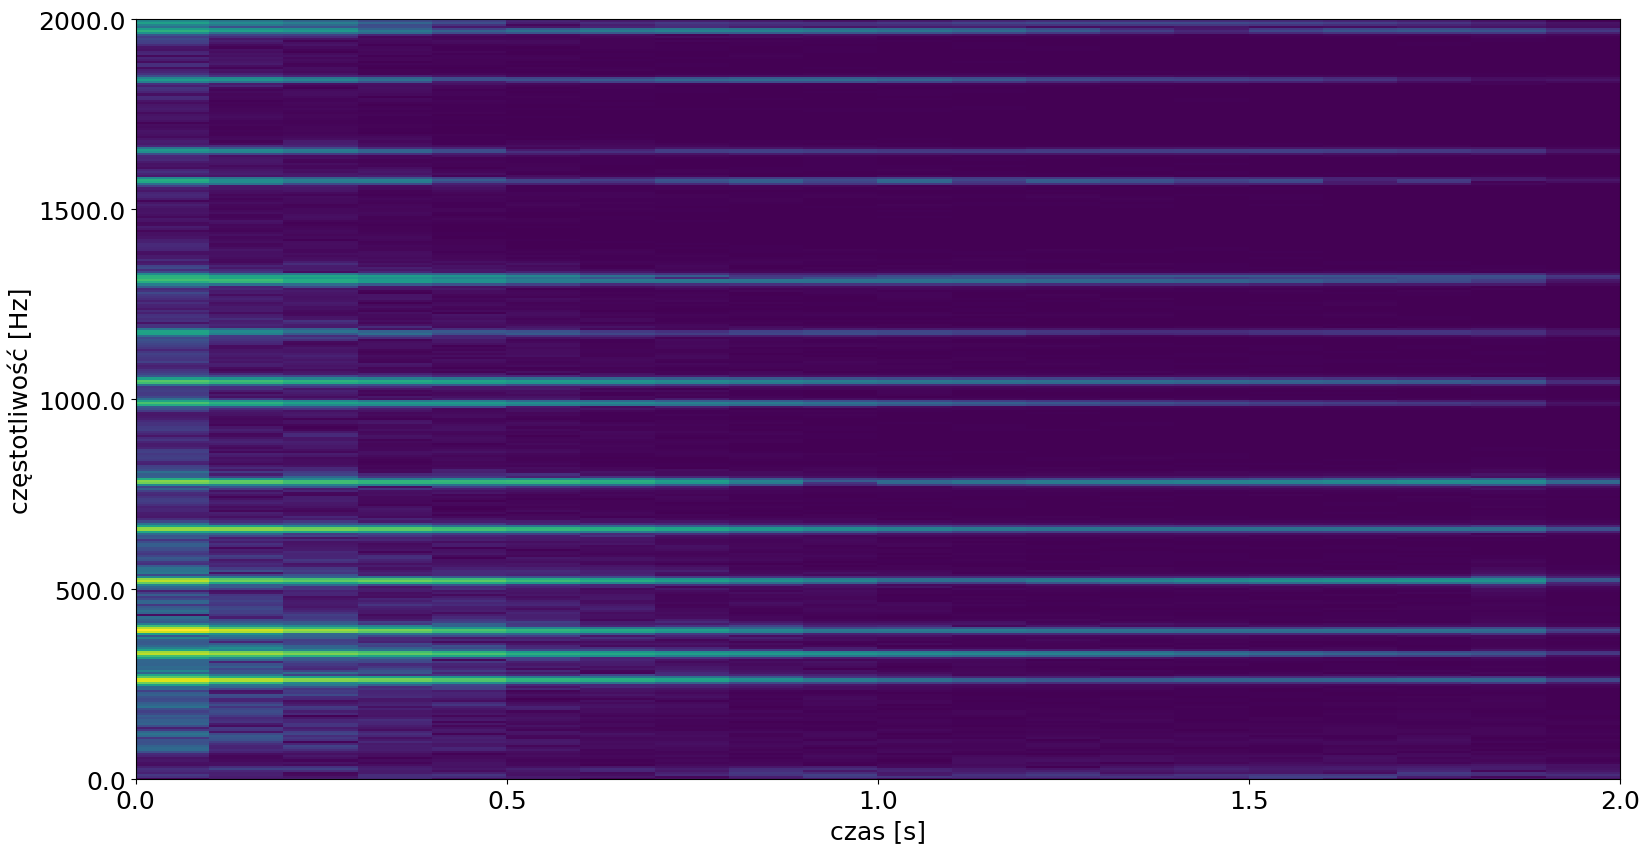
\includegraphics[width=0.9\textwidth]{images/spektrogram_cdur}
    \caption{Spektrogram akordu C-dur zagranego na pianinie.}
    \label{fig:spektrogram_cdur}
\end{figure}



\section{Podstawy analizy akordów muzycznych}

Jak wspominano we wstępie, pierwsze metody analizy akordów muzycznych były oparte jedynie na narzędziach cyfrowego przetwarzania sygnału. Oznacza to, że w~celu zidentyfikowania akordu brzmiącego w~danym fragmencie utworu, wykonywano szereg jasno zdefiniowanych obliczeń, mających na celu rozpoznać, jaki z~predefiniowanej grupy akordów wybrzmiewa w~danej chwili. Metoda tego rodzaju wymaga eksperta znającego się na muzyce oraz matematyce, który przygotuje odpowiedni algorytm na podstawie swojej wiedzy.

Najbardziej oczywiste i~bezpośrednie podejście do tematu analizy akordów przedstawione zostało na schemacie \ref{fig:rozpoznawanie_stare_1}. Dla fragmentu utworu, w~którym chcemy zidentyfikować akord, przeprowadzona zostaje analiza częstotliwościowa (np. DFT). Następnie poszczególne składowe są zamieniane na odpowiadające im nazwy dźwięków (np. $440$ Hz jest zamienianie na dźwięk $a^1$). Ostatecznie na podstawie zbioru reguł wyodrębnione nazwy dźwięków są zamieniane na pewien odpowiadający im akord.

\begin{figure}[htb]
    \centering
    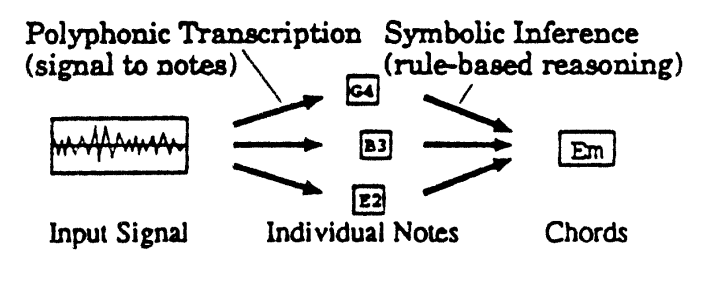
\includegraphics[width=0.9\textwidth]{images/rozpoznawanie_stare_1}
    \caption{Najprostsze podejście do rozpoznawania akordów muzycznych \cite{fujishima_realtime_1999}.}
    \label{fig:rozpoznawanie_stare_1}
\end{figure}

Fujishima \cite{fujishima_realtime_1999} w~swoim artykule z~roku 1999 zaproponował usprawnienie tej metody, wprowadzając strukturę zwaną PCP (ang. \emph{Pitch Class Profile}). Jest to wektor dwunastu wartości, po jednej dla każdego półtonu. Każdy element tego wektora zawiera sumę natężeń składowych sygnału, które odpowiadają danemu dźwiękowi. Po zbudowaniu PCP wykonywany jest odpowiedni algorytm dopasowania wzorców, który ma na celu wybrać ,,najbardziej podobny'' element z~wcześniej zdefiniowanego słownika akordów. Aby więc pomysł mógł zadziałać, wcześniej trzeba przygotować szablon (również w~postaci wektora PCP) dla każdego rodzaju akordu, który chcemy móc zidentyfikować. Cały proces został zaprezentowany na rys. \ref{fig:rozpoznawanie_stare_2}. Zaproponowany tutaj wektor PCP był później wielokrotnie wykorzystywany w~innych pracach, które rozszerzały tę podstawową metodę o~bardziej złożone algorytmy.

\begin{figure}[htb]
    \centering
    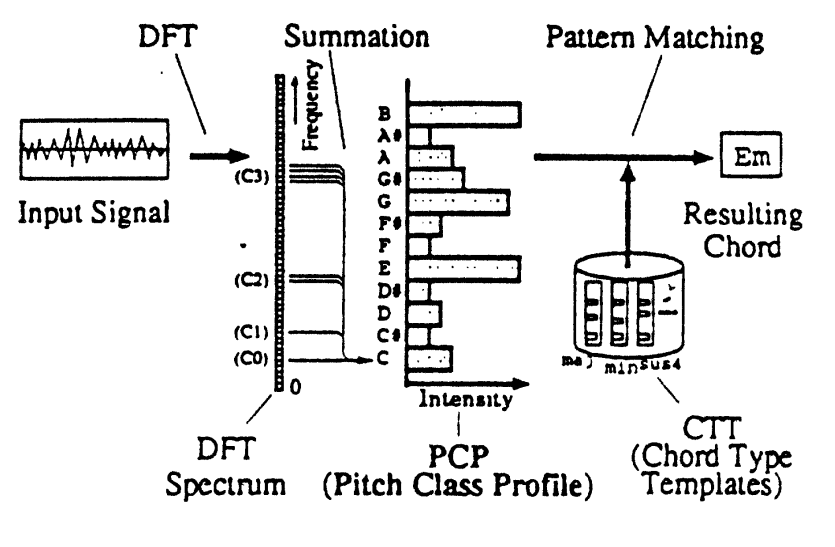
\includegraphics[width=0.9\textwidth]{images/rozpoznawanie_stare_2}
    \caption{Rozpoznawanie akordów muzycznych w~oparciu o~PCP \cite{fujishima_realtime_1999}.}
    \label{fig:rozpoznawanie_stare_2}
\end{figure}
